\documentclass[12pt,a4paper]{article}

% ---------- Basics ----------
\usepackage[utf8]{inputenc}
\usepackage[T1]{fontenc}
\usepackage{lmodern} % ADDED: Better vector fonts
\usepackage[english]{babel}

% ---------- Typography ----------
\usepackage{microtype}
\usepackage[a4paper,margin=2.7cm]{geometry}
\usepackage{setspace}
\setstretch{1.15}

% ---------- Math ----------
\usepackage{amsmath,amssymb}
\usepackage{graphicx}
\usepackage{booktabs}
\usepackage{tabularx}
\usepackage{xurl}

% ---------- Visualization ----------
\usepackage{tikz}
\usetikzlibrary{arrows.meta,positioning,calc}

% ---------- References ----------
% FIX 2: Fix for the babel/polyglossia csquotes warning
\usepackage{csquotes}
\usepackage[
  backend=biber,
  style=alphabetic, % This will output [Author+Year] once Biber compiles successfully
  sorting=ynt,
  maxbibnames=99
]{biblatex}
\addbibresource{references.bib}
\AtEveryBibitem{%
  \clearfield{url}%
  \clearfield{urldate}%
}

% hyperref must generally be the last package loaded...
\usepackage[colorlinks=true,linkcolor=blue,citecolor=blue,urlcolor=blue]{hyperref}

% ...except for cleveref, which must load AFTER hyperref
\usepackage[nameinlink,noabbrev]{cleveref} % ADDED: Smart cross-referencing

% ---------- Front Matter Metadata ----------
\newcommand{\facultyname}{Faculty of Computer Science}
\newcommand{\programname}{Master of Computational Modelling and Simulation}
\newcommand{\reporttype}{Research Project Report}
\newcommand{\reporttitle}{Constructing a Structurally Controlled Benchmark for Relation-Pattern Analysis}
\newcommand{\studentname}{Omar El Ansary}
\newcommand{\matriculationnumber}{5252201}
\newcommand{\studentemail}{omar\_essameldeen\_ahmad.elansary@mailbox.tu-dresden.de}
\newcommand{\supervisorone}{Prof. Dr. Jens Lehmann}
\newcommand{\supervisortwo}{Dr. Kossi Amouzouvi}
\newcommand{\submissiondate}{March 28, 2026}

\title{\reporttitle}
\author{\studentname}
\date{\submissiondate}

\begin{document}
\begin{titlepage}
\centering
\vspace*{1.5cm}
{\Large \facultyname \par}
\vspace{1.4cm}
{\large \programname \par}
\vspace{0.4cm}
{\large \reporttype \par}
\vspace{2.2cm}
{\LARGE\bfseries \reporttitle \par}
\vfill
{\large Supervisors \par}
\vspace{0.3cm}
{\large \supervisorone \par}
{\large \supervisortwo \par}
\vspace{1.4cm}
{\large Submitted by \par}
\vspace{0.3cm}
{\large \studentname \par}
{\large Matriculation Number: \matriculationnumber \par}
{\large \texttt{\studentemail} \par}
\vspace{1.4cm}
{\large Dated \par}
\vspace{0.3cm}
{\large \submissiondate \par}
\end{titlepage}

\clearpage
\thispagestyle{empty}
\section*{Statement of Authorship}
I hereby certify that I have authored this document entitled ``\reporttitle'' independently and without undue assistance from third parties. Only the resources and references indicated in this document have been used. There were no additional persons involved in the intellectual preparation of the present document. I am aware that violations of this declaration may lead to serious consequences.

\vfill
\noindent \studentname \\
\submissiondate

\clearpage
\phantomsection
\addcontentsline{toc}{section}{Abstract}
\begin{abstract}
Knowledge graph benchmarks often exhibit uneven structural relation patterns, making it difficult to separate model behavior from benchmark composition. This thesis presents a modular methodology for constructing a structurally controlled benchmark from Wikidata, focusing on four relation-pattern families: symmetry, anti-symmetry, inversion, and composition.

% TODO before final submission if KGE results arrive:
% revise the next sentence so the abstract reflects both structural audit and downstream evaluation.
The pipeline has two phases. Phase I restricts the relation universe to entity-valued properties, discovers empirically observed two-hop transitions, estimates hop-support statistics, and verifies candidate patterns before converting them into relation-level quotas. Phase II uses these quotas as the reference for graph construction and repair. In the current version, the selected final reported graph is the Stage12 repaired largest component, denoted B0, and the methodology is evaluated on Wikidata primarily through structural audit, while downstream KGE evaluation remains ongoing.

% TODO before final submission if KGE results arrive:
% expand the final sentence below so it does not read as construction-only.
Applied to Wikidata, the selected B0 graph contains 24,683 unique triples across 139 allocated relations in a single weakly connected component. The final reported graph achieves complete coverage of the allocated relation set, but residual pattern imbalance remains, especially for composition-heavy taxonomic relations. The contribution of this thesis in its current form is therefore a Wikidata-instantiated benchmark-construction methodology and audited benchmark instance, not a validated claim of cross-graph generality, perfectly balanced downstream evaluation, or fully resolved end-to-end reproducibility.
\end{abstract}

\clearpage
\phantomsection
\addcontentsline{toc}{section}{Acknowledgements}
\section*{Acknowledgements}
I would like to express my sincere gratitude to \supervisorone{} and \supervisortwo{} for their guidance, feedback, and continued support throughout this research project. Their supervision and discussions were invaluable in shaping the direction of this work and in improving its methodological clarity.

\clearpage
\tableofcontents
\clearpage
\listoffigures
\clearpage
\listoftables
\clearpage

\section{Introduction}
Knowledge graphs represent structured knowledge through entities and relations. Beyond individual triples, relations also exhibit higher-level structural behavior such as symmetry, anti-symmetry, inversion, and composition. These patterns matter for evaluation because knowledge graph embedding (KGE) models are often discussed in terms of the relational behavior they can encode~\cite{sun2019rotate,ali2022bringing}.

Existing benchmark datasets are not structurally neutral. Prior work has shown that benchmark composition and evaluation protocol can materially affect reported performance, and that standard datasets differ substantially in their observed frequencies of structural relation patterns~\cite{sun2020reevaluation,ali2022bringing}. When some pattern families dominate a benchmark while others are scarce, model rankings can reflect benchmark composition as much as reasoning capability.

Related Wikidata-based benchmarks such as CoDEx and InferWiki improve benchmark source quality and inferential design, but they do not explicitly balance structural pattern families within a connected benchmark graph~\cite{safavi2020codex,cao2021inferwiki}.

% TODO before final submission if KGE results arrive:
% soften the benchmark-construction-only framing in this paragraph.
This thesis addresses benchmark construction rather than downstream model training. It aims to construct a connected Wikidata subgraph~\cite{vrandecic2014wikidata} whose triple mass is deliberately allocated across four empirically verified pattern families. Doing so requires pattern discovery at scale, verification under realistic query and retrieval constraints, and graph realization that prevents generic high-support relations from dominating the benchmark.

% TODO before final submission if KGE results arrive:
% if benchmark evaluation is added, update the final sentence to reflect the broader empirical scope.
Our solution is a two-phase pipeline. Phase I restricts attention to entity-valued relations, enumerates empirically observed two-hop transitions, estimates hop support, and verifies symmetric, anti-symmetric, inverse, and compositional behavior before converting accepted candidates into relation-level quotas. Phase II uses these quotas as the reference for graph construction, repair, candidate comparison, and final artifact selection. The reported Wikidata instantiation selects B0, the Stage12 repaired largest component, as the final graph after comparing later nonselected candidate analyses.

Within that scope, this thesis makes four contributions:
\begin{itemize}
    \item an empirical discovery and verification procedure for four structural relation-pattern families;
    \item a relation-level allocation stage that converts verified pattern evidence into integer quotas and an exported support matrix;
    \item a quota-aware graph-construction pipeline combining genericity control, candidate capping, repair, refinement, and connectivity-aware filtering; and
    \item a structural audit of the resulting benchmark, including the failure mode of an abandoned online realization strategy and the residual trade-off between balance and connectivity.
\end{itemize}

The remainder of this thesis is organised as follows. Section~\ref{sec:related-work} reviews related work on benchmark bias and pattern-aware evaluation. Section~\ref{sec:design_and_data} defines the design constraints and data scope. Section~\ref{sec:methodology} presents the benchmark-construction pipeline. Section~\ref{sec:evaluation_discussion} discusses the instantiated benchmark and its limitations. Section~\ref{sec:conclusion} concludes.


\section{Related Work}
\label{sec:related-work}

Research on knowledge graph benchmarks has largely focused on link prediction performance, while the structural composition of benchmark graphs has received less direct control. This is a central issue for the present thesis. The goal here is not only to extract a Wikidata-based benchmark, but to construct one in which structural relation patterns such as symmetry, anti-symmetry, inversion, and composition are represented in a controlled and empirically verified manner. The most relevant prior work can therefore be organized into six lines: benchmark construction and evaluation bias, relation-pattern analysis and rule discovery, Wikidata-specific benchmark construction, graph sampling and connectivity-aware extraction, handling generic relations, and empirical versus logical verification of relation properties.

\paragraph{Benchmark construction and evaluation bias.}
Classic benchmark datasets such as FB15K, FB15K-237, WN18RR, and YAGO3-10 have played a central role in knowledge graph completion research, but they are now well known to have substantial methodological limitations. FB15K and WN18 were shown to contain inverse-relation leakage, which motivated the filtered variants FB15K-237 and WN18RR~\cite{bordes2013transe,toutanova2015observed,dettmers2018conve}. However, removing inverse relations solves only one source of benchmark bias. It does not ensure a balanced distribution of structural relation types, nor does it guarantee that the retained graph remains representative for evaluating structural reasoning.

This concern is reinforced by broader benchmarking studies. Sun et al.\cite{sun2020reevaluation} re-evaluated knowledge graph completion methods and showed that methodological details strongly affect reported performance. Ali et al.~\cite{ali2022bringing} extended this concern by demonstrating that model performance is highly dependent not only on the interaction function, but also on training approach, loss function, and explicit inverse-relation modeling. Their study is especially relevant here because it includes a dedicated relational-pattern analysis over FB15K-237, WN18RR, and YAGO3-10, showing that benchmark datasets differ substantially in their observed frequencies of symmetry, anti-symmetry, and composition~\cite{ali2022bringing}. The key limitation, relative to this thesis, is that these works diagnose benchmark bias after dataset construction. They do not construct a benchmark whose triple mass is explicitly allocated across structural pattern families.

\paragraph{Relation-pattern analysis and rule discovery.}
A second relevant line of work concerns how relation patterns are identified. Rule mining systems such as AMIE~\cite{galarraga2013amie} and AnyBURL~\cite{meilicke2019anyburl} extract Horn-style rules from incomplete knowledge graphs and provide an interpretable alternative to latent embedding models. These systems are important because they operationalize notions such as inversion and composition through empirical support in observed graph structure. InferWiki explicitly relies on AnyBURL to generate train/test splits in which test triples are inferable from training data~\cite{cao2021inferwiki}. This makes InferWiki one of the strongest comparison targets for work that emphasizes empirical structural reasoning.

A different but related direction is pattern-centered benchmark design. Sadeghi et al.~\cite{sadeghi2021relational} construct datasets targeted at specific graph relational patterns and study model behavior across those settings. This is highly relevant conceptually, because it shows that evaluation should distinguish between different structural regimes instead of treating all triples as interchangeable. However, those datasets isolate patterns into separate evaluation scenarios. They do not build a single connected benchmark graph in which multiple pattern families coexist under controlled allocation constraints. That is precisely the gap addressed here.

\paragraph{Wikidata-specific benchmark construction.}
Because this thesis constructs a benchmark from Wikidata, prior Wikidata-based benchmarks are particularly important. Wikidata itself provides the underlying knowledge source and data model~\cite{vrandecic2014wikidata}. CoDEx is one of the most important benchmark papers in this space. It extracts benchmark graphs from Wikidata and Wikipedia, improves over older Freebase-centered datasets, and analyzes logical relation patterns in the resulting graphs~\cite{safavi2020codex}. It is a strong baseline for comparison because it is Wikidata-based, multi-domain, and explicitly motivated by benchmark quality rather than only raw scale.

InferWiki is even closer to the present thesis in one respect: it is also Wikidata-based and is explicitly designed around inferential structure rather than random splitting~\cite{cao2021inferwiki}. Its contribution is to ensure that test samples are supported by training-side reasoning paths. However, its primary objective is inferential predictability and open-world evaluation, not balanced construction across relation-pattern families. Likewise, large-scale benchmarks such as WikiKG90Mv2 prioritize scale and realistic temporal splitting over structural control~\cite{hu2021ogblsc,ogb_wikikg90mv2}. They are therefore valuable contextual baselines, but not direct methodological competitors.

\paragraph{Graph sampling, subgraph extraction, and connectivity-aware construction.}
Most benchmark construction pipelines implicitly rely on some graph extraction strategy, even when that strategy is not the main scientific contribution. CoDEx uses seeded collection and subsequent $k$-core filtering to produce denser benchmark subgraphs~\cite{safavi2020codex}. This is important because it shows that benchmark quality depends not only on relation choice but also on graph topology. Similarly, the OGB line acknowledges that large knowledge graphs often have highly skewed relation distributions and must be subsampled carefully for evaluation~\cite{hu2021ogblsc,ogb_wikikg90mv2}.

Nevertheless, existing extraction strategies still stop short of the requirements of this thesis. They do not jointly optimize for relation retention, pattern-family balance, fragmentation control, and connected benchmark construction. In other words, prior work samples subgraphs for tractability or difficulty, whereas this thesis samples under structural allocation constraints. That difference is methodologically substantial.

\paragraph{Handling generic and hub relations.}
Another recurring issue in benchmark design is the presence of highly generic, high-degree, or hub-like relations. Such relations can dominate graph connectivity and triple mass while contributing limited discriminatory value for structural evaluation. This issue appears implicitly in several benchmark papers. CoDEx reduces noise and sparsity through filtering~\cite{safavi2020codex}. WikiKG90Mv2 explicitly notes that raw validation and test triples are highly skewed toward a few relations and therefore applies relation balancing during subsampling~\cite{ogb_wikikg90mv2}. More broadly, studies on benchmark realism and reproducibility have shown that performance gains may partly arise from structural shortcuts rather than genuine reasoning ability~\cite{akrami2018reevaluating,akrami2020realistic,sun2020reevaluation,ali2022bringing}.

However, prior work typically addresses this problem indirectly, either by removing obvious leakage relations or by downsampling dominant relations. It does not formalize a benchmark construction stage in which genericity itself acts as a constraint on allocation and graph realization. The present thesis contributes exactly at this point by treating genericity as a construction risk that must be controlled together with fragmentation and relation retention.

\paragraph{Empirical versus logical verification of relation properties.}
Finally, this thesis is positioned at the boundary between logical and empirical views of relation properties. Some datasets inherit logical assumptions from schema or curated rule sets, whereas others infer relation behavior directly from observed graph evidence. Ali et al.~\cite{ali2022bringing} define symmetry, anti-symmetry, inversion, and composition using support and confidence, explicitly acknowledging knowledge graph incompleteness. InferWiki also follows an empirical perspective by mining rules from observed data rather than assuming closed logical axioms~\cite{cao2021inferwiki}. This perspective is especially suitable for Wikidata, where many structurally important regularities are not available as clean logical declarations but can still be observed in the graph.

The current thesis follows this empirical line, but pushes it further into benchmark construction itself. Rather than merely analyzing pattern frequencies after extraction or using rules only for split generation, the pipeline estimates hop support, prunes and verifies candidate composition targets, and allocates graph mass accordingly. The resulting contribution is therefore not just another Wikidata benchmark. It is a benchmark-construction pipeline that treats structural pattern balance as a first-class design objective.

\paragraph{Summary of the gap.}
Taken together, prior work establishes four important facts. First, benchmark choice strongly shapes conclusions about model quality. Second, structural patterns such as symmetry, inversion, and composition are unevenly distributed across standard datasets. Third, Wikidata offers a richer and more current source than older Freebase-centered resources. Fourth, rule-based and empirical analyses reveal structural regularities that conventional random extraction ignores. What remains insufficiently addressed is the construction of a connected Wikidata-based benchmark in which structural relation-pattern families are explicitly identified, verified, balanced, and realized under graph-level constraints. This unresolved gap directly motivates the benchmark design proposed in this thesis.

\section{Benchmark Design and Data Scope}
\label{sec:design_and_data}

Before detailing the general computational pipeline proposed in this thesis, it is necessary to establish the operational boundaries of our chosen source graph. While the core two-phase methodology is designed to be database-agnostic, any practical deployment must adapt to the scale, schema, and infrastructure of the target knowledge base. To demonstrate the framework's efficacy, we instantiate it in this work using Wikidata. Consequently, this section formalizes the specific design constraints, API limitations, and exact data scope extracted from Wikidata to feed the construction pipeline.

\subsection{Design Constraints and System Assumptions}

The architecture of the proposed pipeline is shaped by dataset, infrastructure, and methodological constraints that directly affect source selection, candidate discovery, and final graph construction. This section formalizes those constraints and distinguishes literature-backed premises from thesis-specific design requirements.

% ---------------------------------------------------------
\subsubsection{Dataset Selection Constraints}

\paragraph{Choice of Wikidata.}

Wikidata was selected as the source knowledge graph because it is openly accessible, broad in topical coverage, and large enough to expose a wide range of relation types and structural behaviors \cite{hosseini2024wikidata_subsetting}. Wikidata also provides public dumps, a public SPARQL endpoint, and property-level metadata that can be exploited during benchmark construction \cite{hosseini2024wikidata_subsetting,wikidata_constraints_portal,wikidata_inverse_constraint}.

At the property level, Wikidata currently lists more than $13{,}000$ properties on its public property index \cite{wikidata_list_properties_2025}. In addition, Wikidata maintains community-defined property constraints, including subject- and value-type guidance as well as inverse-property constraints, which are useful as weak semantic signals during search-space reduction \cite{wikidata_constraints_portal,wikidata_inverse_constraint}. These constraints are not treated as hard logical guarantees, but they remain practically useful for pruning implausible candidates.

Alternative sources such as DBpedia were less suitable for the present objective. DBpedia is constructed by extracting structured content from Wikipedia and mapping it to a shared ontology \cite{lehmann2015dbpedia}. In the classic DBpedia ontology design, that shared ontology contains 320 classes and 1,650 properties \cite{lehmann2015dbpedia}. Relative to Wikidata, this yields a substantially smaller and more schema-constrained relation space, which is less favorable for large-scale structural pattern discovery.

Widely used benchmark datasets such as FB15k, FB15k-237, WN18, and WN18RR were also not appropriate as source graphs. They are already benchmark subsets created for downstream evaluation rather than source corpora for benchmark construction. Moreover, the original FB15k and WN18 are known to suffer from inverse-relation leakage, which motivated the creation of FB15k-237 and WN18RR as reduced variants with inverse relations removed \cite{toutanova2015observed,dettmers2018conve}. Since the goal of this thesis is to construct a structurally balanced benchmark from a richer source graph, pre-filtered benchmark subsets are not an appropriate starting point.

\paragraph{Scale as a Computational Constraint.}

The same scale that makes Wikidata attractive also makes exhaustive structural discovery impractical. With approximately $1.3 \times 10^4$ listed properties \cite{wikidata_list_properties_2025}, naive enumeration already yields the following candidate counts:

\[
|R| \approx 1.3 \times 10^4
\]

\[
|R|^2 \approx 1.69 \times 10^8
\]

\[
|R|^3 \approx 2.2 \times 10^{12}
\]

Even before empirical verification, exhaustive testing of all relation pairs and triples would therefore require evaluating hundreds of millions to trillions of candidate combinations. This combinatorial growth is a mathematical consequence of the relation inventory itself and does not require a separate citation.

The size of Wikidata further strengthens this constraint. Recent work reports more than 100 million data items and more than 1.4 billion statements for Wikidata as of January 2023 \cite{hosseini2024wikidata_subsetting}. For the purposes of this thesis, the exact count is less important than the order of magnitude: the graph is sufficiently large that brute-force structural enumeration is not methodologically or computationally realistic.

Accordingly, the scale of Wikidata is both an asset and a constraint. It provides the structural breadth required for pattern discovery, but it also necessitates aggressive candidate-space reduction before empirical verification.

% ---------------------------------------------------------
\subsubsection{Infrastructure and Querying Constraints}

\paragraph{Use of WDQS Instead of Full Dumps.}

A full local materialization of Wikidata was not practical within the computational scope of this thesis. Prior work on Wikidata subsetting reports that the JSON dump of 14 December 2022 was 112\,GB in compressed form and cites hardware recommendations on the order of 16 vCPUs, 128\,GB memory, and 800\,GB SSD storage for maintaining a local copy \cite{hosseini2024wikidata_subsetting}. Current official dump listings also show that Wikidata dumps remain in the hundred-gigabyte range in compressed form \cite{wikidata_dumps_2026}. In addition, the Wikidata Query Service (WDQS) user manual notes that importing the full dump into a query-service setup can take about 12 days, followed by additional time to catch up the update lag \cite{wikidata_query_service_manual}.

For that reason, this thesis relies on the publicly available Wikidata Query Service (WDQS) instead of building a full local warehouse. This is a scope decision: the emphasis is benchmark construction methodology, not engineering a production-grade local Wikidata infrastructure.

\paragraph{SPARQL Endpoint Limitations.}

Using WDQS introduces endpoint-specific constraints that directly shape the discovery strategy. The public WDQS documentation states a hard query deadline of 60 seconds, a per-client budget of 60 seconds of processing time per 60-second window, a limit of 30 error queries per minute, and a limit of five parallel queries per IP; clients exceeding these limits are throttled with HTTP 429 responses \cite{wikidata_query_service_manual}. As a consequence, large Cartesian joins over broad predicate sets, deep multi-hop expansions, and overly aggressive concurrent querying are not suitable default strategies on the public endpoint.

These constraints motivate the use of staged discovery, controlled batching, checkpointing, and reuse of cached intermediate results. The decision to avoid exhaustive predicate enumeration is therefore not merely an optimization choice; it follows directly from the operational properties of the public query infrastructure.

\paragraph{Concurrency Constraints.}

Because WDQS throttling is applied at the client level, parallel requests issued from the same client identity still contribute to a shared processing budget \cite{wikidata_query_service_manual}. In practice, this means that naive multithreading does not provide unlimited throughput and can instead increase the likelihood of throttling. For this reason, metadata enrichment and discovery outputs are cached locally once retrieved, and repeated live queries are avoided whenever deterministic reuse is possible.

% ---------------------------------------------------------
\subsubsection{Methodological Constraints}

\paragraph{Restriction to Selected Relational Patterns.}

This thesis restricts attention to four relation-pattern families: symmetry, antisymmetry, inversion, and composition. These patterns are standard in the knowledge graph embedding literature and are especially relevant because geometric relation representations have been explicitly analyzed with respect to symmetry, antisymmetry, inversion, and composition behavior \cite{sun2019rotate}. They also align with the benchmark objective of evaluating whether models behave differently across structurally distinct relation types.

More expressive logical phenomena, such as longer rule chains or general Horn-rule families, are intentionally excluded. Their discovery and verification would enlarge the candidate space substantially and would require a different methodological scope. This restriction is therefore a thesis design decision motivated by tractability and benchmark focus, not a claim that longer rules are unimportant in general.

\paragraph{Empirical Reduction Requirement.}

Only empirically observed two-hop transitions are considered during discovery. This is a thesis-specific design decision introduced to reduce the candidate space before verification. It ensures that relation-pair analysis is grounded in observed graph structure rather than in all theoretically possible predicate combinations.

\paragraph{Semantic Compatibility Pruning.}

Even after empirical reduction, the composition search space remains large. For that reason, semantic compatibility pruning is applied before expensive verification steps. In this thesis, compatibility signals derived from Wikidata property constraints are used as weak filters rather than as hard ontology axioms \cite{wikidata_constraints_portal,wikidata_inverse_constraint}. The pruning policy itself is a design choice of the proposed pipeline.

% ---------------------------------------------------------
\subsubsection{Structural Construction Constraints}

\paragraph{Connectivity Requirement.}

The final benchmark graph is required to be connected. This should be understood as a benchmark-design requirement of this thesis, not as a universally established rule for all knowledge graph benchmarks. The purpose of this requirement is to avoid producing a benchmark that decomposes into many unrelated islands, which would weaken the interpretation of downstream structural evaluation.

\paragraph{Structural Balance Requirement.}

The primary benchmark objective is to mitigate relation-pattern bias. Therefore, the extracted subgraph is required to contain a comparable amount of evidence across the selected structural pattern families. This is again a thesis-specific design requirement. It follows from the evaluation goal of comparing model behavior under more controlled structural exposure rather than from an external standard benchmark recipe.

\paragraph{Interpretation of empirical confidence estimates.}

Confidence values in this thesis should be interpreted as empirical shortcut rates over the retrieved and examined chain instances, not as formal logical guarantees over the full knowledge graph. Wilson intervals quantify uncertainty conditional on the examined sample, but they do not remove bias introduced by upstream retrieval effects such as endpoint truncation, pagination limits, or query-time constraints.

\paragraph{Reproducibility Constraint.}

All metadata enrichment and structural discovery outputs are cached and serialized. This is a procedural design constraint introduced to reduce repeated dependence on live endpoint variability and to make the benchmark construction process reproducible under the same cached inputs.

% =========================================================
\subsection{Data Source and Relation Scope}

Wikidata properties span heterogeneous datatypes, including entity-valued properties, literal-valued attributes, identifiers, temporal values, quantities, media links, and structural metadata \cite{vrandecic2014wikidata}. Our benchmark focuses on relation patterns that are expressed through multi-hop connectivity over entities. We therefore restrict the initial analysis to properties whose values are Wikidata items (i.e., properties with the datatype \texttt{wikibase-item}).

This restriction is a strict methodological requirement grounded in graph theory and standard embedding formulations, rather than a mere technical convenience. In standard knowledge graph embedding frameworks, models are mathematically defined to operate over a relational graph $\mathcal{G} \subseteq \mathcal{E} \times \mathcal{R} \times \mathcal{E}$, where both the head and tail are entities ($\mathcal{E}$) capable of forming further connections \cite{sun2019rotate,ali2022bringing}. 

Conversely, non-entity values---such as strings, dates, or numerical quantities---act as terminal leaf nodes in the graph topology. Because a literal value cannot act as the subject of a new outgoing edge, it cannot serve as the intermediate bridging node $y$ in a composition path $x \xrightarrow{r_1} y \xrightarrow{r_2} z$. Furthermore, terminal nodes cannot participate in the closed directed cycles required to define symmetry or inversion. Therefore, restricting the universe to \texttt{wikibase-item} properties ensures that the pipeline does not waste computational budget evaluating structural rules on identifier properties, measurement attributes, or maintenance metadata, concentrating the benchmark exclusively on relations for which multi-hop structural reasoning is semantically and mathematically possible.

\paragraph{Initial Candidate Universe and Metadata.}
The initial candidate universe is derived from Wikidata ontology metadata. After excluding non-entity-valued properties, the resulting relation set contains approximately 1,700 candidate relations \cite{wikidata_list_properties_2025}. 

For each retained relation, we collect essential metadata to be used in later pruning, verification, and analysis stages. This includes the English label and description, aliases, domain and range constraints, declared inverse properties, and example triples \cite{wikidata_constraints_portal,wikidata_inverse_constraint}. 

\paragraph{Empirical interpretation.}
Throughout the pipeline, support and confidence measures are interpreted empirically, aligning with the Open World Assumption (OWA) inherent to knowledge graphs. All values are computed exclusively from the evidence retrieved under the chosen querying procedure; missing evidence is treated as a lack of observed support rather than as a formal proof of a universal logical failure. This interpretation (conceptually similar to the Partial Completeness Assumption utilised in rule mining \cite{galarraga2013amie}) ensures that scores reflect observed behaviour, not formal guarantees over the full Wikidata knowledge graph.

\section{Methodology}
\label{sec:methodology}

Operating on the constrained data scope established in Section~\ref{sec:design_and_data}, the benchmark construction workflow is organized into two primary phases. Phase I identifies empirical relation patterns and computes relation-level quotas. Phase II then uses these quotas to build a concrete graph under a suite of structural constraints. 

\subsection{Phase I: Empirical Target Filtering and Allocation Pipeline}

Building on the constrained relation universe of approximately 1,700 \texttt{wikibase-item} properties established previously, Phase I maps these candidates to actionable target quotas. As illustrated in Figure~\ref{fig:Phase1_pipeline}, this phase consists of successive discovery, support-estimation, pruning, verification, and allocation stages.

\begin{figure}[!htbp]
\centering
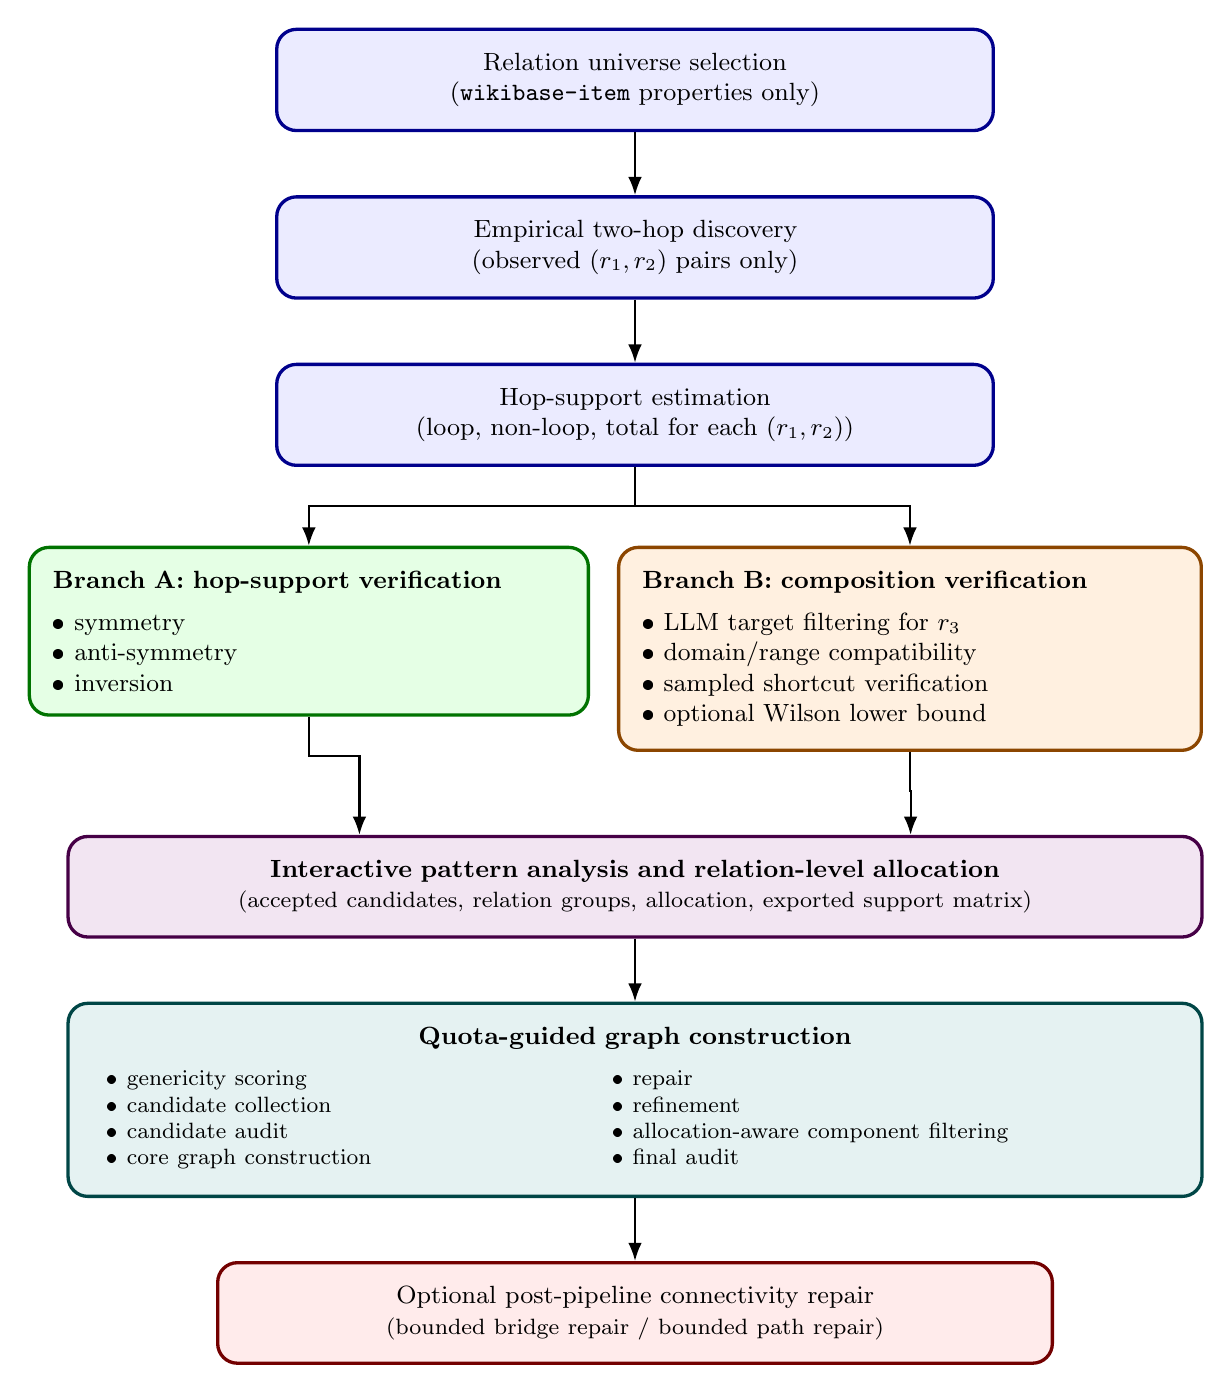
\begin{tikzpicture}[
    node distance=8mm and 5mm, % Tighter horizontal spacing between branches
    >=Latex,
    basebox/.style={
        draw,
        rounded corners=2.5mm,
        very thick,
        font=\small,
        inner sep=3mm % This provides the internal padding so text never touches the border
    },
    mainbox/.style={
        basebox,
        align=center,
        text width=8.5cm, 
        fill=blue!8,
        draw=blue!55!black
    },
    branchAbox/.style={
        basebox,
        align=left,
        text width=6.5cm, % 6.5cm + 6.8cm + 0.5cm gap = 13.8cm (Fits single column perfectly)
        fill=green!10,
        draw=green!45!black
    },
    branchBbox/.style={
        basebox,
        align=left,
        text width=6.8cm,
        fill=orange!12,
        draw=orange!55!black
    },
    allocbox/.style={
        basebox,
        align=center,
        text width=13.8cm, 
        fill=violet!10,
        draw=violet!55!black
    },
    graphbox/.style={
        basebox,
        align=center,
        text width=13.8cm,
        fill=teal!10,
        draw=teal!55!black
    },
    optionalbox/.style={
        basebox,
        align=center,
        text width=10cm,
        fill=red!8,
        draw=red!45!black
    },
    arrow/.style={->, thick}
]

% --- NODES ---
\node[mainbox] (scope)
{Relation universe selection\\(\texttt{wikibase-item} properties only)};

\node[mainbox, below=of scope] (discovery)
{Empirical two-hop discovery\\(observed $(r_1,r_2)$ pairs only)};

\node[mainbox, below=of discovery] (support)
{Hop-support estimation\\(loop, non-loop, total for each $(r_1,r_2)$)};

% Verification Branches (Placed precisely relative to support node)
\node[branchAbox, below left=10mm and -40mm of support] (branchA)
{\textbf{Branch A: hop-support verification}\\[1.5mm]
\textbullet~symmetry\\
\textbullet~anti-symmetry\\
\textbullet~inversion};

\node[branchBbox, below right=10mm and -48mm of support] (branchB)
{\textbf{Branch B: composition verification}\\[1.5mm]
\textbullet~LLM target filtering for $r_3$\\
\textbullet~domain/range compatibility\\
\textbullet~sampled shortcut verification\\
\textbullet~optional Wilson lower bound};

% Allocation
\node[allocbox, below=15mm of support |- branchA.south] (alloc)
{\textbf{Interactive pattern analysis and relation-level allocation}\\
\footnotesize (accepted candidates, relation groups, allocation, exported support matrix)};

% Graph Construction
\node[graphbox, below=of alloc] (graph)
{\textbf{Quota-guided graph construction}\\[2mm]
\footnotesize
\begin{tabular}{@{}p{6cm} p{7cm}@{}}
\textbullet~genericity scoring & \textbullet~repair \\
\textbullet~candidate collection & \textbullet~refinement \\
\textbullet~candidate audit & \textbullet~allocation-aware component filtering \\
\textbullet~core graph construction & \textbullet~final audit
\end{tabular}};

\node[optionalbox, below=of graph] (repair)
{Optional post-pipeline connectivity repair\\
\footnotesize (bounded bridge repair / bounded path repair)};

% --- CONNECTIONS ---
\draw[arrow] (scope) -- (discovery);
\draw[arrow] (discovery) -- (support);

% Branching connections
\draw[arrow] (support.south) -- ++(0,-0.5) -| (branchA.north);
\draw[arrow] (support.south) -- ++(0,-0.5) -| (branchB.north);

% Merging connections
\draw[arrow] (branchA.south) -- ++(0,-0.5) -| ([xshift=-3.5cm]alloc.north);
\draw[arrow] (branchB.south) -- ++(0,-0.5) -| ([xshift=3.5cm]alloc.north);

\draw[arrow] (alloc) -- (graph);
\draw[arrow] (graph) -- (repair);

\end{tikzpicture}
\caption[Phase I benchmark-construction workflow]{Overall benchmark-construction workflow. After restricting the relation universe to entity-valued Wikidata properties, the pipeline first discovers empirically observed two-hop relation pairs and computes hop-support statistics. From this point, the workflow branches: symmetry, anti-symmetry, and inversion are verified directly from hop-support counts, whereas composition is handled through a separate target-pruning and shortcut-verification branch. The accepted pattern candidates are then merged in the allocation stage, whose outputs drive the final quota-guided graph-construction pipeline. Optional post-pipeline connectivity-repair operators are available for residual fragmentation but are not native stages of the main reported workflow.}
\label{fig:Phase1_pipeline}
\end{figure}

% ---------------------------------------------------------
\subsubsection{Stage 1: Empirical Two-Hop Discovery}

Instead of enumerating all $(r_1, r_2)$ pairs, we query Wikidata to retrieve only empirically observed two-hop paths:
\[
(x, r_1, y) \wedge (y, r_2, z)
\]
For each $r_1$, we obtain the set:
\[
\mathrm{ValidR2}(r_1)
\]
This step reduces the theoretical $|R|^2$ space to empirically supported transitions. In practice, this yields approximately 340,000 observed pairs. 
This reduction removes only relation pairs that were not observed during the discovery stage.

% ---------------------------------------------------------
\subsubsection{Stage 2: Support Estimation}

For each source relation $r_1$ and each candidate second-hop relation $r_2$, we estimate support over distinct two-hop paths of the form
\[
x \xrightarrow{r_1} y \xrightarrow{r_2} z.
\]
To exclude trivial self-loop artifacts, we retain only nontrivial paths satisfying
\[
x \neq y
\qquad\text{and}\qquad
y \neq z.
\]
Let $T$ denote the set of triples in the queried graph, and let
\[
\mathcal{P}(r_1,r_2)
=
\left\{
(x,y,z)\;\middle|\;
% \begin{aligned}
(x,r_1,y)\in T, %\\
(y,r_2,z)\in T, %\\
x \neq y,\; y \neq z
% \end{aligned}
\right\}
\]
be the set of observed nontrivial two-hop paths for the ordered pair $(r_1,r_2)$. We then define loop, non-loop, and total support as
\[
S_{\mathrm{loop}}(r_1,r_2)
=
\left|
\left\{
(x,y,z)\in \mathcal{P}(r_1,r_2)
\;\middle|\;
x=z
\right\}
\right|,
\]
\[
S_{\mathrm{non}}(r_1,r_2)
=
\left|
\left\{
(x,y,z)\in \mathcal{P}(r_1,r_2)
\;\middle|\;
x\neq z
\right\}
\right|,
\]
\[
S_{\mathrm{tot}}(r_1,r_2)
=
S_{\mathrm{loop}}(r_1,r_2)
+
S_{\mathrm{non}}(r_1,r_2).
\]
% Here, $S_{\mathrm{loop}}$, $S_{\mathrm{non}}$, and $S_{\mathrm{tot}}$ denote loop, non-loop, and total support, respectively.
Thus, Stage 2 produces, for each ordered pair $(r_1,r_2)$, empirical loop, non-loop, and total support counts over observed nontrivial two-hop paths. The counting is performed over distinct observed two-hop witnesses $(x,y,z)$ rather than only over endpoint pairs $(x,z)$, so different intermediate entities $y$ contribute separately when they instantiate distinct two-hop paths. 
These raw support values are written out by the extraction stage without imposing a support cutoff. A minimum support threshold $\tau$ is applied later, during the downstream analysis stage, in order to suppress weakly supported relation pairs, stabilize empirical confidence estimates, and reduce noise in pattern selection.


From this point, the workflow branches. One branch uses the hop-support counts directly to evaluate symmetric, anti-symmetric, and inverse behavior. The other branch is specific to composition: it combines the observed $(r_1,r_2)$ pairs with a pruned set of candidate target relations $r_3$ and performs separate composition verification. The outputs of both branches are then merged in the interactive pattern-analysis and allocation stage.

% ---------------------------------------------------------
\subsubsection{Stage 3: Composition Target Pruning}

Even after reducing the observed two-hop relation pairs $(r_1,r_2)$, composition still requires choosing which target relations $r_3 \in R$ are worth testing. Unlike symmetry, anti-symmetry, and inversion, composition introduces a third relation and therefore a much larger candidate space. We therefore apply an additional pruning stage only for composition. Its purpose is not to prove that a relation is compositional, but to remove targets for which composition testing is structurally or semantically unlikely to be useful.

\paragraph{LLM-Based Composition-Target Filtering}

The first pruning step uses an LLM as a high-recall semantic triage classifier for candidate target relations $r_3$. For each relation, the model receives structured metadata describing the relation, including its label, description and other available property metadata collected previously, and is asked only whether the relation is a plausible \emph{target} of a two-hop composition rule of the form
\[
r_1(a,b) \wedge r_2(b,c) \Rightarrow r_3(a,c).
\]
The classifier does not choose the composing relations $r_1,r_2$ and does not attempt to prove composition. Its task is only to decide whether testing the relation as a composition target is worthwhile.

To reduce hallucination risk and over-pruning, the prompt was designed conservatively. The model was restricted to a binary decision: either the relation is worth testing as a target or it is \texttt{NO\_WAY}. The \texttt{NO\_WAY} label was intended to be used sparingly and only when testing would be structurally or semantically wasted. When uncertain, the model was instructed to keep the relation rather than discard it. The prompt also explicitly framed composition as a definitional shortcut relation and excluded explanatory, provenance, attribute-propagation, and terminal classification-style relations from positive target decisions. Thus, the LLM was used only as a coarse semantic filter with high recall, not as an oracle for logical validity.

Relations classified as implausible composition targets were removed from further composition testing. This reduced the target-relation set from approximately 1700 to approximately 615. This filtering step was applied only to composition target selection and did not affect the candidate sets for symmetry, anti-symmetry, or inversion.

Operationally, relation triage was implemented by a batched OpenAI classification pipeline over the relation-profile collection. For each relation, the payload contained the relation identifier, label, description, datatype, domain type IDs, range type IDs, and, when available, a bounded number of example triples and aliases. Relations whose datatype was not \texttt{wikibase-item} were excluded before any LLM call and assigned \texttt{composition\_target = NO\_WAY} automatically. The remaining relations were sent to the OpenAI chat-completions API in batches of \(20\) by default, with JSON-schema-constrained output, temperature \(0.2\), and up to three retry attempts under exponential backoff. The prompt explicitly framed the task as high-recall triage rather than proof: for composition, the model was instructed to decide only whether the relation was worth testing as the target of a two-hop composition rule, and to output \texttt{composition\_target} in \(\{\texttt{YES},\texttt{NO\_WAY}\}\) together with a short \texttt{composition\_reason}, choosing \texttt{YES} under uncertainty. The same response schema also stored symmetry, anti-symmetry, and inverse triage labels, but the downstream composition-target enrichment stage used only \texttt{llm\_classification.composition.composition\_target} and retained every relation whose value was not \texttt{NO\_WAY}. The script defaulted to model \texttt{gpt-4.1-mini}, although this could be overridden at runtime via \texttt{--model}. The resulting classifications were persisted back to MongoDB under the field \texttt{llm\_classification}. The current implementation does not document a manual review or composition-specific post-hoc correction step.

\paragraph{Domain and Range Compatibility for Composition Targets}

The second pruning step applies domain and range compatibility constraints to the remaining composition candidates. Its purpose is to reduce the space of tested triples $(r_1,r_2,r_3)$ before empirical composition verification. 
For a candidate composition target $r_3$, we require compatibility between the start type of the composed path and the domain of the target relation, and between the end type of the composed path and the range of the target relation:
\[
\begin{aligned}
\mathrm{Dom}(r_1) \cap \mathrm{Dom}(r_3) &\neq \emptyset,\\
\mathrm{Rng}(r_2) \cap \mathrm{Rng}(r_3) &\neq \emptyset.
\end{aligned}
\]
A candidate triple $(r_1,r_2,r_3)$ is removed only when the available type declarations are explicitly incompatible. If one side is unknown or has no declared types, that side is treated as unconstrained and does not by itself eliminate the candidate. In other words, empty or missing domain/range information is interpreted permissively rather than as evidence of incompatibility. This avoids discarding candidates purely because ontology metadata are incomplete.

This compatibility pruning is also applied only to composition and does not modify the candidate sets for symmetry, anti-symmetry, or inversion.

% ---------------------------------------------------------
\subsubsection{Stage 4: Pattern Verification Branches} 
The extracted hop-support counts are then reused in two verification branches. 
The first branch uses the hop-support counts directly to evaluate symmetric, anti-symmetric, and inverse behavior.

\paragraph{Hop-Support-Based Verification of Symmetry, Anti-symmetry, and Inversion.}

(\textbf{Symmetric Confidence}) 
For a relation $r$, symmetric behavior is evaluated on the self-pair $(r,r)$. The empirical symmetric confidence is defined as
\[
\mathrm{conf}_{\mathrm{sym}}(r)
=
\frac{S_{\mathrm{loop}}(r,r)}
{S_{\mathrm{tot}}(r,r)}.
\]

\paragraph{Anti-symmetric Confidence} 
For the same self-pair $(r,r)$, anti-symmetric behavior is estimated as the complementary proportion of non-return paths:
\[
\mathrm{conf}_{\mathrm{anti}}(r)
=
\frac{S_{\mathrm{non}}(r,r)}
{S_{\mathrm{tot}}(r,r)}.
\]
Since
\[
S_{\mathrm{tot}}(r,r)
=
S_{\mathrm{loop}}(r,r) 
+
S_{\mathrm{non}}(r,r),
\]
this can equivalently be written as
\[
\mathrm{conf}_{\mathrm{anti}}(r)
=
1-\mathrm{conf}_{\mathrm{sym}}(r).
\]
% Thus, symmetric confidence measures the extent to which repeated application of $r$ returns to the starting entity, whereas anti-symmetric confidence measures the extent to which it does not.


\paragraph{Inverse Confidence} 
For an ordered pair $(r_1,r_2)$, the forward inverse-style confidence is estimated as
\[
\mathrm{conf}_{\mathrm{inv}}^{\rightarrow}(r_1,r_2)
=
\frac{S_{\mathrm{loop}}(r_1,r_2)}
{S_{\mathrm{tot}}(r_1,r_2)}.
\]
The reverse-direction score is computed analogously on the reversed ordered pair:
\[
\mathrm{conf}_{\mathrm{inv}}^{\leftarrow}(r_1,r_2)
=
\frac{S_{\mathrm{loop}}(r_2,r_1)}
{S_{\mathrm{tot}}(r_2,r_1)}.
\]
These two directional scores are not assumed to be equal. To require reciprocal consistency, the final inverse confidence is defined conservatively as
\[
\mathrm{conf}_{\mathrm{inv}}(r_1,r_2)
=
\min\!\left(
\mathrm{conf}_{\mathrm{inv}}^{\rightarrow}(r_1,r_2),
\mathrm{conf}_{\mathrm{inv}}^{\leftarrow}(r_1,r_2)
\right).
\]
This choice ensures that a relation pair receives a high inverse score only when both directions exhibit strong return behavior.


\paragraph{Composition Verification} 
The second branch is specific to composition. Unlike symmetry, anti-symmetry, and inversion, composition is not verified directly from the hop-support output alone, because it additionally requires a candidate shortcut relation $r_3$ for each observed pair $(r_1,r_2)$.

\paragraph{Composition Confidence} 
For a candidate rule
\[
(r_1,r_2) \Rightarrow r_3,
\]
we consider sampled chain instances of the form
\[
x \xrightarrow{r_1} y \xrightarrow{r_2} z,
\]
and test whether the shortcut triple
\[
x \xrightarrow{r_3} z
\]
is also present. 
Let
\[
N_{\mathrm{exam}}(r_1,r_2,r_3)
\]
denote the number of examined chain pairs for the candidate triple $(r_1,r_2,r_3)$, and let
\[
N_{\mathrm{hit}}(r_1,r_2,r_3)
\]
denote the number of examined chain pairs for which the shortcut relation $r_3$ is observed. The empirical composition confidence is then defined as
\[
\mathrm{conf}_{\mathrm{comp}}(r_1,r_2,r_3)
=
\frac{N_{\mathrm{hit}}(r_1,r_2,r_3)}
{N_{\mathrm{exam}}(r_1,r_2,r_3)}.
\]

Thus, composition confidence is an empirical shortcut frequency over sampled verified chains, not a direct function of the phase-1 loop/non-loop support counts. In the dashboard, this quantity is loaded from the compact composition-verification output and may optionally be refined by Wilson-score lower-bound filtering before candidate acceptance.



\subsubsection{Stage 5: Interactive Pattern Analysis and Allocation}


The interactive pattern-analysis pipeline serves as the integration point at which the empirically verified pattern candidates are brought together and converted into relation-level allocations. Its main role in the reported workflow is to take the accepted symmetric, anti-symmetric, inverse, and composition candidates, organize them into relation groups, and compute the allocation on demand. The resulting allocated relations and exported relation-level support matrix are then passed to the graph-construction pipeline described in the following section.

This stage distinguishes between two relation-level matrices with different roles. First, it constructs a raw relation--relation support matrix whose entries are aggregated pair-support totals. Second, it transforms this matrix into an allocation matrix that determines how support contributes to quota assignment. This distinction is methodologically important because raw support magnitudes alone can cause a small number of high-support relations to dominate the allocation. In the reported experiments, allocation used the \texttt{log1p\_balanced\_norm} transformation, which compresses heavy-tailed support values and balances row-wise and column-wise structural influence before computing allocation probabilities.

Operationally, let \(A\) denote the filtered Phase-I relation-support matrix whose entries are aggregated pair-support totals. Under \texttt{log1p\_balanced\_norm}, the dashboard first applies the elementwise transform
\[
W_0 = \log(1 + A).
\]
It then computes a row-normalized matrix
\[
W^{\mathrm{row}}_{ij} = \frac{(W_0)_{ij}}{\sum_k (W_0)_{ik}}
\]
and a column-normalized matrix
\[
W^{\mathrm{col}}_{ij} = \frac{(W_0)_{ij}}{\sum_k (W_0)_{kj}},
\]
using zero-safe division when a row or column sum is zero. The final allocation matrix is
\[
W = \tfrac{1}{2}\left(W^{\mathrm{row}} + W^{\mathrm{col}}\right).
\]
This transformed matrix is the one passed into the bidirectional allocator. In the dashboard it is the recommended default for quota allocation. Later graph-building stages do not have to reuse this same transformation: the dashboard exports a separate genericity/support matrix over the positive-\(\eta\) relation set, and the downstream pipeline configuration recommends the direct-support mode \texttt{adjacency\_support} for that export.


\paragraph{Relation-group construction and bidirectional allocation.}
After filtering the candidate pattern outputs, the accepted candidates are collapsed to unique relation-level groups for the four target pattern families. %: symmetric, anti-symmetric, inverse, and composition. 
This conversion is necessary because the upstream analyses operate on different objects, such as ordered relation pairs for inversion and ordered relation triples for composition, whereas the allocation stage assigns mass to individual relations.

Let $A \in \mathbb{R}_{\ge 0}^{m \times m}$ denote the filtered relation--relation support matrix over the active relation universe $\mathcal{R}=\{r_1,\dots,r_m\}$, where each entry $A_{ij}$ stores the aggregated stage-1 pair-support total for the ordered pair $(r_i,r_j)$ after support thresholding. The allocation does not operate directly on $A$, but on a transformed matrix $W=f(A)$. In the reported experiments, we use the \texttt{log1p\_balanced\_norm} transformation, which compresses extreme support values and balances row-wise and column-wise influence.

For each pattern group $G$ with target budget $\eta_G$, the allocator computes, for every relation $r \in G$, a forward score from the row-sum of $W$ restricted to $G$ and a backward score from the corresponding column-sum. These two directional scores are converted into softmax probabilities and averaged, yielding a relation-specific allocation weight. The expected allocation for relation $r$ is then obtained by multiplying this averaged probability by the total group budget $\eta_G$, after which an integerized quota is derived. Consequently, relations that are more strongly integrated into the support structure of their pattern group receive a larger share of the group budget, while the total allocated mass remains constrained by the user-specified group target
\begin{align*}
s_f(r) &= \sum_{r' \in G} W_{rr'}, &
s_b(r) &= \sum_{r' \in G} W_{r'r},\\
% \end{align*}
% \begin{align*}
P_f(r\mid G,W)
&=
\frac{\exp(s_f(r))}
{\sum_{\tilde r \in G}\exp(s_f(\tilde r))}, &
P_b(r\mid G,W)
&=
\frac{\exp(s_b(r))}
{\sum_{\tilde r \in G}\exp(s_b(\tilde r))},\\
% \end{align*}
% \begin{align*}
p_{\mathrm{avg}}(r)
&=
\frac{1}{2}\bigl(P_f(r\mid G,W)+P_b(r\mid G,W)\bigr), &
\eta^{\mathrm{expected}}_r
&=
\eta_G \, p_{\mathrm{avg}}(r).
\end{align*}
The final integer quota is obtained by applying the selected integerization procedure to the expected allocations. 
Operationally, integerization is applied after the real-valued expected allocations \(\eta^{\mathrm{expected}}_r\) have been computed for each relation in a pattern group. When integerization is enabled, the allocator uses Hamilton's largest-remainder method. For each relation \(r\), it first computes the base allocation
\[
b_r = \left\lfloor \eta^{\mathrm{expected}}_r \right\rfloor.
\]
Let
\[
R_G = \eta_G - \sum_r b_r
\]
be the remaining number of units to distribute for a group with total budget \(\eta_G\). If \(R_G > 0\), the remaining units are assigned one-by-one to the relations with the largest fractional remainders
\[
\eta^{\mathrm{expected}}_r - \left\lfloor \eta^{\mathrm{expected}}_r \right\rfloor.
\]
Ties are resolved deterministically. In the dashboard call path no custom tie-break order is supplied, so equal fractional parts fall back to the relation order induced by the group list. The implementation also contains a defensive overshoot branch for the case \(R_G < 0\), in which units are removed from the smallest fractional parts while preserving non-negativity. The final integer allocation vector is asserted to sum exactly to the original group budget \(\eta_G\). In the dashboard, integerization is enabled by default.

\paragraph{Exported support matrix for the graph-construction pipeline.}
Beyond the matrix used for allocation, the pipeline also constructs a second relation-level matrix over the subset of relations with positive integer allocation. This exported matrix is used by the graph-construction pipeline described in the following section, where a support representation restricted to the actually allocated relations is required. Its role is therefore different from that of the allocation matrix: it is not used to determine quotas, but to provide a relation--relation support view for later genericity-aware and graph-construction decisions. In the configuration used in this work, this matrix preserves direct support semantics through the \texttt{adjacency\_support} representation, so that the later pipeline operates on raw support magnitudes rather than on the transformed allocation weights.

\subsubsection{Summary of Phase I.}
In summary, the first phase of the methodology successfully transitions from a theoretical, unconstrained relation universe to a concrete, empirically verified foundation. By discovering observed paths, pruning unviable targets, and rigorously verifying structural patterns, the pipeline distills the data into two actionable outputs: an integer target quota ($\eta_r$) for each accepted relation and an exported relation-level support matrix. These outputs serve as the direct blueprint for the subsequent graph-generation phase.


\subsection{Phase II: Quota-Aware Graph Construction and Refinement}

The allocation stage produces, for each selected relation \(r\), an integer target quota \(\eta_r\). These quotas are used as the reference for graph construction and for auditing candidate outputs. The intended Phase II design is an eight-stage quota-aware graph-construction workflow, illustrated in Figure \ref{fig:Phase2_pipeline}, but the final reported artifact is stated more conservatively: the selected final graph is B0, the Stage12 repaired largest component.

Direct attempts to convert allocated quotas into a connected graph using online, frontier-based SPARQL sampling (further analyzed in Section~\ref{sec:abandoned-allocation}) revealed a mismatch between relation-level planning and entity-level feasibility. In particular, binary relation existence under live WDQS did not translate into sufficient attach capacity under the connectivity invariant of the growing graph.

To resolve these bottlenecks, the Phase II design moves away from online attach-only sampling toward a quota-aware candidate-pool strategy:
\begin{itemize}
    \item \textbf{Solving the Local Bottleneck:} Stage 2 is designed to retrieve a bounded candidate pool for each relation \emph{before} rigid graph-building constraints are applied.
    \item \textbf{Preventing Generic Dominance:} Stage 1 identifies taxonomic hubs, while Stage 4 actively penalizes hub-dominated candidates to ensure narrower relations can be realized.
    \item \textbf{Preventing Fragmented Loss:} Stage 7 removes structurally weak components conservatively, while retaining small components that preserve the unique core realization of a relation with positive allocation.
\end{itemize}

\begin{figure}[!htbp]
\centering
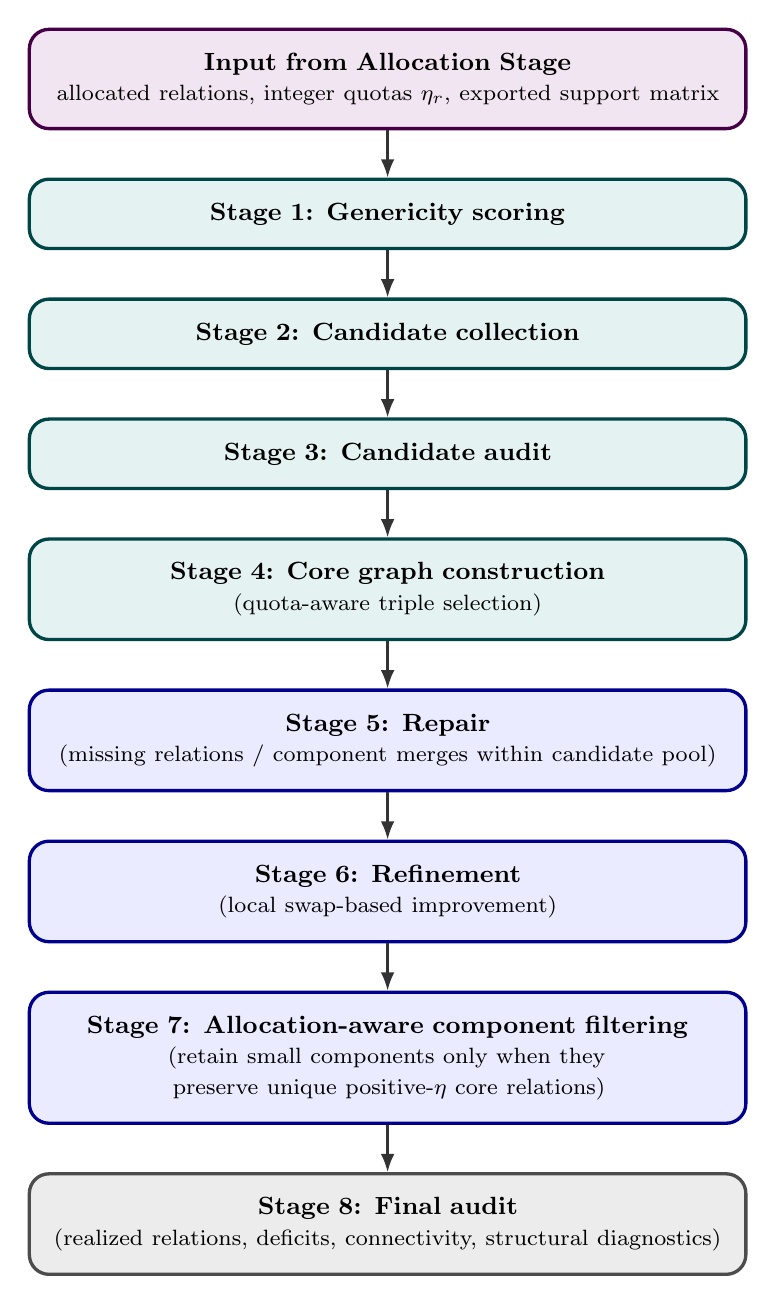
\begin{tikzpicture}[
    node distance=6mm,
    >=Latex,
    basebox/.style={
        draw,
        rounded corners=2.5mm,
        very thick,
        align=center,
        text width=8.5cm, % Ensures uniform width and automatic text wrapping
        inner sep=3mm,
        font=\small
    },
    % Color themes mapped to Phase X
    inputbox/.style={basebox, fill=violet!10, draw=violet!55!black},
    corebox/.style={basebox, fill=teal!10, draw=teal!55!black},
    refinebox/.style={basebox, fill=blue!8, draw=blue!55!black},
    auditbox/.style={basebox, fill=gray!15, draw=gray!60!black},
    arrow/.style={->, thick, draw=black!80}
]

% Nodes
\node[inputbox] (input) {\textbf{Input from Allocation Stage}\\
\footnotesize allocated relations, integer quotas $\eta_r$, exported support matrix};

\node[corebox, below=of input] (g1) {\textbf{Stage 1: Genericity scoring}};
\node[corebox, below=of g1] (g2) {\textbf{Stage 2: Candidate collection}};
\node[corebox, below=of g2] (g3) {\textbf{Stage 3: Candidate audit}};
\node[corebox, below=of g3] (g4) {\textbf{Stage 4: Core graph construction}\\
\footnotesize (quota-aware triple selection)};

\node[refinebox, below=of g4] (g5) {\textbf{Stage 5: Repair}\\
\footnotesize (missing relations / component merges within candidate pool)};
\node[refinebox, below=of g5] (g6) {\textbf{Stage 6: Refinement}\\
\footnotesize (local swap-based improvement)};
\node[refinebox, below=of g6] (g7) {\textbf{Stage 7: Allocation-aware component filtering}\\
\footnotesize (retain small components only when they preserve unique positive-\(\eta\) core relations)};

\node[auditbox, below=of g7] (g8) {\textbf{Stage 8: Final audit}\\
\footnotesize (realized relations, deficits, connectivity, structural diagnostics)};

% Connections
\draw[arrow] (input) -- (g1);
\draw[arrow] (g1) -- (g2);
\draw[arrow] (g2) -- (g3);
\draw[arrow] (g3) -- (g4);
\draw[arrow] (g4) -- (g5);
\draw[arrow] (g5) -- (g6);
\draw[arrow] (g6) -- (g7);
\draw[arrow] (g7) -- (g8);

\end{tikzpicture}
\caption[Phase II quota-guided graph-construction design]{Quota-guided graph-construction design after relation-level allocation. The allocation stage provides integer quotas per relation together with an exported relation-support matrix. The intended graph-construction workflow first scores genericity, collects and audits relation-wise candidate triples, and then builds a quota-aware core graph. Subsequent repair and refinement stages operate within the collected candidate pool. Finally, an allocation-aware component filter removes structurally weak fragments while retaining small components that preserve unique core realizations of relations with positive allocation, after which a final audit computes graph-level and relation-level diagnostics. The selected reported artifact is B0, the Stage12 repaired largest component, rather than a claim that every intended offline stage is fully reproducible end-to-end from frozen inputs.}
\label{fig:Phase2_pipeline}
\end{figure}

\subsubsection{Stage 1: Genericity Scoring}

The first stage assigns each allocated relation a genericity score that reflects how structurally broad or hub-like the relation is in the exported relation-support matrix. The score combines relation coverage, support mass, candidate-volume proxies, and manually identified structural-risk indicators. Relations are then grouped into low-, medium-, and high-genericity buckets. This information is not used to discard relations, but to shape later candidate collection and scoring so that very generic relations do not dominate the constructed graph.

Operationally, the genericity score is computed for the currently allocated relation set, using the exported genericity support matrix together with the integer allocation results. For each allocated relation \(r\), the pipeline computes a coverage score
\[
\mathrm{coverage}(r)
=
\frac{
\left|
\left\{
c \in \mathcal{R}_{\mathrm{alloc}}
\;\middle|\;
M_{rc} > \varepsilon_s
\;\lor\;
M_{cr} > \varepsilon_s
\right\}
\right|
}{
\max(1, |\mathcal{R}_{\mathrm{alloc}}|)
},
\]
where \(M\) denotes the exported genericity support matrix and \(\varepsilon_s\) is the genericity support threshold. It also computes the raw support mass
\[
\mathrm{support\_mass}(r)
=
\sum_{c \in \mathcal{R}_{\mathrm{alloc}}} (M_{rc} + M_{cr}),
\]
a normalized mass score
\[
\mathrm{mass\_score}(r)
=
\frac{\mathrm{support\_mass}(r)}{\max_{u \in \mathcal{R}_{\mathrm{alloc}}} \mathrm{support\_mass}(u)},
\]
and a candidate-volume proxy
\[
\mathrm{vol\_score}(r)
=
\frac{\eta_r}{\max_{u \in \mathcal{R}_{\mathrm{alloc}}} \eta_u}.
\]
In addition, a manual structural-risk flag is defined as
\[
\mathrm{manual}(r)
=
\begin{cases}
1, & r \in \mathcal{R}_{\mathrm{manual}},\\
0, & \text{otherwise.}
\end{cases}
\]
The final genericity score is then
\[
\mathrm{genericity\_score}(r)
=
0.35\,\mathrm{coverage}(r)
+
0.25\,\mathrm{mass\_score}(r)
+
0.20\,\mathrm{vol\_score}(r)
+
0.20\,\mathrm{manual}(r).
\]

Let \(q_{0.90}\) denote the empirical \(0.90\)-quantile of the raw support-mass values over the allocated relations. Bucket assignment is then performed as follows. A relation is placed in the high-priority genericity screening branch whenever \(\mathrm{manual}(r)=1\), or \(\mathrm{coverage}(r)\ge \tau_{\mathrm{cov}}\), or \(\mathrm{support\_mass}(r)\ge q_{0.90}\). Within that branch, the relation is assigned to the \texttt{high} bucket if \(\mathrm{genericity\_score}(r)\ge 0.60\) or \(\mathrm{manual}(r)=1\), and to \texttt{medium} otherwise. Outside that branch, the relation is assigned to \texttt{medium} if \(\mathrm{genericity\_score}(r)\ge 0.33\), and to \texttt{low} otherwise. In the inspected configuration, the default manual-risk relation set is \(\{ \texttt{P31}, \texttt{P279}, \texttt{P131}, \texttt{P17} \}\), the support threshold is \(10^{-12}\), the coverage threshold is \(0.80\), and the top-mass quantile is \(0.90\).

\subsubsection{Stage 2: Candidate Collection}

For each allocated relation \(r\), the intended design retrieves a bounded candidate set of concrete triples. The target number of collected candidates is determined from the allocated quota \(\eta_r\) through a quota-aware rule with floor and cap constraints. Candidate collection is performed relation-wise and is adapted to the genericity bucket of the relation: highly generic relations are treated more conservatively, while small candidate sets may be retained in full. In the final reporting, this stage is described as part of the Phase II design rather than as evidence that the complete offline execution path can be reproduced exactly without resolving the remaining provenance and environment gaps.

\subsubsection{Stage 3: Candidate Audit}

The collected candidates are then audited relation-wise. This audit measures candidate count, entity diversity, concentration, and related statistics that help identify undercollected or overly concentrated relations before graph construction begins. This stage is diagnostically important because it reveals whether some relations are already difficult to realize before structural filtering is applied.

\subsubsection{Stage 4: Core Graph Construction}

The core graph is built by selecting triples from the candidate pool under a quota-aware scoring function. The score rewards relations that still have unmet quota, encourages first realization of previously unrealized relations, and favors triples that improve attachability and component merging. It also penalizes hub-dominated, generic, and noisy candidates. Thus, graph construction is neither purely quota-driven nor purely structural: it jointly optimizes relation realization and graph quality.

Formally, if \(\mathcal{G}_{\mathrm{sel}}\) denotes the current selected graph and \(c_r(\mathcal{G}_{\mathrm{sel}})\) denotes the number of currently selected triples of relation \(r\), then the construction objective prefers triples that improve quota fulfillment while increasing connectivity and limiting undesirable structural concentration. The output of this stage is the first concrete graph instantiating the allocated relation quotas.

\subsubsection{Stage 5: Repair}

After core construction, a repair stage attempts to realize relations that remain missing and to merge disconnected components using still-unused candidates. This stage remains quota-aware: it does not overfill relations that are already at or above their intended target.

\subsubsection{Stage 6: Refinement}

The refinement stage performs bounded local improvements through swap-based search. Its objective is lexicographic: maximize the number of realized relations, reduce total relation deficit, reduce fragmentation, and improve graph quality. In this way, refinement operates as a local post-construction improvement step rather than as a new graph-building phase.

\subsubsection{Stage 7: Allocation-Aware Component Filtering}

After refinement, the graph may still contain many structurally weak connected components. Standard graph-theoretic approaches, such as naive Largest Connected Component (LCC) extraction or size-based pruning, risk indiscriminately removing triples from already underfilled relations, thereby destroying relation fidelity \cite{leskovec2006sampling}. 

For this reason, the implemented workflow uses an allocation-aware weak-component filter rather than naive Largest Connected Component extraction or size-only pruning. A connected component is marked as small if either its triple count falls below \(\tau_{\mathrm{triples}}\) or its entity count falls below \(\tau_{\mathrm{entities}}\). Such a component is removed unless it contains at least one relation \(r\) for which the current core graph contains exactly one core realization and the allocation for that relation satisfies \(\eta_r > 0\). In that case the entire component is retained as a structurally weak exception, and its triples are flagged accordingly. Thus, the implemented preservation mechanism is a binary component-level keep/drop rule with a unique-core-relation exception, not a per-relation eta-derived safety floor. In the inspected configuration, the default weak-component thresholds are \(\tau_{\mathrm{triples}} = 3\) and \(\tau_{\mathrm{entities}} = 3\).

\subsubsection{Stage 8: Final Audit}

The final stage computes graph-level and relation-level audit statistics on the filtered graph. These include the total number of selected triples, number of entities, number of connected components, realized allocated relations, unrealized allocated relations, and related structural indicators. This stage provides the final benchmark-level diagnostics used to interpret the output of the graph-construction pipeline.

% =========================================================
\subsection{Post-Pipeline Connectivity Repair}

In addition to the intended eight-stage graph-construction workflow, the framework includes connectivity-repair operators: a bounded bridge-repair procedure (\texttt{bridge-repair}) and a bounded path-repair procedure (\texttt{path-repair}).

These operators address a strict limitation of the candidate-pool design. Stages 5 through 7 operate over the harvested candidate pool; they can merge components only when suitable connecting triples already exist among the harvested candidates. Consequently, if a disconnected fragment can only be reattached by querying new, external evidence, the native candidate-pool workflow cannot resolve it. The selected final graph B0 is the Stage12 repaired largest component produced after this repair process. This selection should be read as a documented artifact decision, not as a claim that the full upstream Phase II execution has been proven exactly reproducible from frozen inputs.

\paragraph{Bounded Bridge Repair.} 
The bridge-repair utility is a conservative post-processing operator that attempts to reconnect a non-largest weakly connected component to the main graph through a one-hop or two-hop bridge. By selecting anchor nodes from disconnected components, querying Wikidata for neighboring triples, and accepting only bridge candidates that satisfy active eta-safety criteria, it provides a minimal-intervention recovery method. It improves connectivity through short, interpretable bridges without inflating the graph unnecessarily.

\paragraph{Bounded Path Repair.} 
The path-repair utility generalizes the bridge approach to short, multi-hop paths. Instead of testing only one- or two-hop reconnections, it performs a constrained search from anchor nodes, subject to explicit limits on hop count, search expansions, newly introduced entities, and admissible non-core edges. 

\paragraph{The Cost-Safety Trade-off.}
Although bounded path repair is strictly more expressive than bounded bridge repair, we retain the two operators as separate methods rather than collapsing them into a single procedure. Methodologically, they occupy different points in the cost--safety--auditability trade-off. Bridge repair acts as the conservative baseline: it is cheaper to run, easier to interpret, and highly controlled. Path repair provides the necessary expressive power when direct bridge repair fails, but at the cost of increased computational expense and higher sensitivity to policy choices. Preserving this distinction allows future users to choose the repair strategy that best fits their computational budget and strictness requirements.

% =========================================================
\subsection{Possible Adaptation to Other Target Graphs}
\label{sec:generalization}

Although the methodology detailed above is instantiated on Wikidata, some components are modular enough that they could in principle be adapted to other multi-relational knowledge bases, such as DBpedia, YAGO, or proprietary enterprise graphs. This thesis does not empirically validate cross-graph transfer, so the discussion below should be read as an adaptation note rather than as a demonstrated generalization claim.

Because Phase I handles data ingestion while Phase II handles quota allocation and graph construction, the later stages are less tied to Wikidata than the upstream retrieval and metadata stages.
\begin{enumerate}
    \item \textbf{Redefine the Relation Scope:} Replace the \texttt{wikibase-item} restriction with the target ontology's corresponding object-property definition. In DBpedia, this would be \texttt{owl:ObjectProperty}.
    \item \textbf{Map Semantic Constraints:} Replace Wikidata's property constraint portal with the target graph's native schema constraints (e.g., standard RDFS domain and range declarations) to inform the Phase I composition pruning stage.
    \item \textbf{Adjust Collection Ceilings:} Calibrate the Phase II candidate-collection parameters and API throttling limits to match the specific infrastructure capacity and query-timeout rules of the target graph's endpoint.
\end{enumerate}
These requirements indicate a plausible adaptation path, but they do not by themselves establish that the full methodology transfers unchanged across target graphs.

\section{Evaluation and Discussion}
\label{sec:evaluation_discussion}

Having established the two-phase benchmark construction pipeline, this section evaluates the structural outcomes of the methodology. We first analyze an alternative, online graph-construction strategy to demonstrate the fundamental topological challenges of frontier-based sampling. We then evaluate the selected B0 graph to assess its relation coverage and allocation fidelity.

The Abandoned Online branch is interpreted here primarily as a negative experimental branch. Its post-hoc audit used an earlier allocation manifest than the selected B0 and later balance-pruning analyses, so exact fulfillment metrics are not strictly like-for-like across all three artifacts. The most direct comparison remains structural behavior, broad pattern pressure, and the qualitative feasibility of connected realization.

% ---------------------------------------------------------
\subsection{Analysis of Alternative Construction Strategies: Online SPARQL Realization}
\label{sec:abandoned-allocation}

Before adopting the quota-guided construction pipeline, we briefly explored an online approach to translate relation-level allocations into a connected entity-level graph. The aim was to instantiate each allocated relation~$r$ by sampling concrete triples $(h,r,t)$ from Wikidata such that the resulting graph matched the allocated quotas \(\eta_r\) while remaining connected throughout its construction.

\subsubsection{Objective and Mechanism}
The procedure separated \emph{allocation} from \emph{realization}. Allocation determined how many triples each relation should contribute. Realization attempted to materialize these quotas by issuing SPARQL queries to the Wikidata Query Service on a relation-by-relation basis. A growing frontier of entities~$V$ was maintained. A candidate triple \((h,r,t)\) was accepted only if it attached to the current frontier (i.e., $h \in V \lor t \in V$). This attach-only rule was intended to enforce connected growth by construction. In the implemented branch, initial feasibility was effectively a binary existence check at the relation level: a relation could pass this precheck by existing somewhere in WDQS even if it later proved difficult to attach under the current connected component.


\subsubsection{Observed Failure Mode: The Realization Collapse}
Despite its simplicity, this design failed to achieve the intended coverage. In the most informative Abandoned Online checkpoint considered here, the realized graph reached \(4{,}026\) triples and \(85\) appearing relations. Under the earlier allocation manifest used for Abandoned Online, \(125\) relations carried positive quota, of which \(40\) never appeared in the extracted graph, and the postprocessed graph remained fragmented across \(162\) weak components. Although this improved over earlier online settings, it still realized only about one fifth of the intended \(20{,}000\)-triple mass. The experiment therefore exposed a strict mismatch between relation-level planning and graph-local feasibility: relation-level allocation and graph-level realization are not equivalent under a connected, type-constrained extraction procedure.

\subsubsection{Topological Bottlenecks and Sampling Bias}
Post-extraction audits revealed several structural factors contributing to this collapse:

\paragraph{Allocation does not imply realizability.} A positive quota does not guarantee that an instance attaches to the current graph. Realization requires that some triple of~$r$ connects to~$V$, which may never happen if \(r\)'s instances lie in disconnected regions of the global graph.

\paragraph{Binary feasibility was too weak.} In the online branch, passing the initial feasibility screen meant only that a relation existed somewhere in WDQS. This was far weaker than showing that the relation could be filled at quota scale while preserving connected growth. As a result, many relations that were globally present still had zero or negligible immediate attach capacity under the current frontier.

\paragraph{Graph-local realizability bottleneck.} Post-run analysis indicated that the run did not mainly fail through one terminal stall followed by unsuccessful rescue. Instead, it kept making shallow progress on a subset of relations while many others repeatedly showed no useful attach capacity under the evolving component. Coverage-first selection improved breadth only partially, but did not converge toward an allocation-faithful connected graph.

\noindent This should be interpreted as evidence from the reported runs rather than as a formal impossibility result for every frontier-based realization scheme.

\paragraph{Frontier-based sampling bias.} The attach-only rule makes the procedure heavily path-dependent. Early sampling decisions strongly influence which relations can later be realized. Similar to Snowball sampling or Breadth-First Search (BFS) in network measurement, frontier-based exploration is known to severely bias samples towards high-degree nodes and depend heavily on the traversal frontier \cite{kurant2010bias, leskovec2006sampling}.

\paragraph{Fragmentation and weak coverage.} Independent relation-wise retrieval did not ensure sufficient overlap among entity sets. In the Abandoned Online postprocessed graph, this yielded \(162\) weak components, even though approximately \(71.46\%\) of entities still lay in the largest connected component.

\paragraph{Generic-relation dominance.} Relations with extremely broad support, such as \texttt{instance of}~(P31) and \texttt{subclass of}~(P279), were much easier to realize under frontier constraints. In the realized graph, these taxonomic relations dominated the connected backbone, while narrower relations remained unrealized.

\subsubsection{Methodological Conclusion}
The experiment showed that a frontier-constrained, attach-only realization is unsuitable for the benchmark-construction objective pursued here as a main production strategy. Even with relaxed settings, the branch yielded only a shallow partial realization rather than an allocation-faithful connected graph. This failure also cannot be attributed simply to a broader positive-eta relation set in Abandoned Online: its documented manifest allocated 125 unique positive-eta relations, whereas the later B0 and balance-pruning artifacts were audited under a 139-relation manifest. This yields an important methodological lesson: online, frontier-based sampling conflicts strongly with strict relation-level quota allocation. Relation mass must be collected with more independence from immediate attachability, a finding that motivated the quota-aware candidate-pool design. Additional online variants with more permissive settings were also explored, but they did not alter the same qualitative failure mode: connected live realization remained under-fulfilled and structurally insufficient for use as the final reported graph.

% ---------------------------------------------------------
\subsection{Structural Evaluation of the Constructed Benchmark}
\label{sec:discussion}

Having justified the departure from online sampling, we now evaluate the structural properties of the selected final reported graph.

\subsubsection{Allocation Fidelity in the Selected B0 Graph}
To assess allocation fidelity, we examined B0, the Stage12 repaired largest component selected as the final reported graph. B0 contains \(24{,}683\) unique triples, \(21{,}893\) unique entities, and \(139\) unique relations in a single weakly connected component. All \(139\) allocated relations are represented and no allocated relation has zero realized triples, overcoming the primary failure mode of the abandoned SPARQL approach. However, the quotas are not evenly satisfied: only 41 relations meet or exceed their allocated targets (of which 17 are exactly fulfilled and 24 are overfilled), while 98 relations remain underfilled. Relative to the expected allocation of \(20{,}000\), B0 therefore exhibits a surplus of \(6{,}702\) and a deficit of \(2{,}019\).

\subsubsection{Pattern Imbalance and the Connectivity Tradeoff}
Pattern-level analysis revealed a pronounced imbalance. When relation counts were apportioned back to structural patterns, the realized triple counts were approximately \(4{,}970\) for anti-symmetric relations, \(11{,}267\) for composition, \(4{,}824\) for inverse, and \(3{,}622\) for symmetric relations. Given a uniform target of \(5{,}000\) per pattern, composition was overrepresented and symmetry was underrepresented. 

Most of the overrepresentation is concentrated in a few high-frequency composition relations. In particular, \texttt{instance of}~(P31) alone contributes nearly six thousand triples, exceeding its target by more than an order of magnitude. This confirms that while the selected B0 graph achieves complete relation coverage, taxonomic backbone relations remain so structurally pervasive that achieving perfect allocation balance without fracturing the graph remains exceedingly difficult.

To isolate this tension, we conducted a diagnostic balance-pruning ablation where the graph was aggressively pruned to enforce strict allocation balance. While this ablation removed most of the overall surplus (reducing total surplus from \(6{,}702\) to \(105\)) and largely corrected the composition overrepresentation (from a surplus of \(6{,}267\) to a deficit of \(297\)), it resulted in severe structural collapse, reducing the largest connected component to 14.0\% of the graph's nodes across 5,623 weak components. This strict ablation is therefore not the final graph.

Table~\ref{tab:quantitative_comparison} quantitatively contrasts Abandoned Online, the selected B0 graph, and the strict balance-pruned ablation. Because the Abandoned Online row is audited against an earlier allocation manifest, it should be read primarily as a structural and broad-pressure comparison rather than as a strictly like-for-like fulfillment benchmark against the later graph variants. Even under that caveat, the comparison illustrates the central structural trade-off in the construction problem: relation balance cannot be forced strictly without sacrificing global connectivity.

After B0, additional graph candidates were evaluated as post hoc analyses rather than as replacements for the final graph. The Stage13/C1 \texttt{aggressive\_but\_guarded} pruning candidate reduced graph size and total surplus relative to B0, but increased total deficit. A deletion-only targeted generic-pruning candidate, C2, preserved weak connectivity and relation coverage but failed the predefined surplus threshold and was rejected as a final candidate. A subsequent \texttt{C3\_probe\_v1} feasibility probe tested remove-and-replace feasibility using an eligible replacement pool; it did not generate a graph candidate and found no feasible replacements for the tested connectivity-critical bridge-like target edges. These analyses did not supersede B0 as the selected final reported graph.


\begin{table}[htbp]
\centering
\small
\setlength{\tabcolsep}{4pt}
\caption[Quantitative comparison of graph variants]{Quantitative comparison of Abandoned Online, the selected B0 Stage12 largest component, and the strict balance-pruned ablation. The Abandoned Online row is reported against an earlier allocation manifest and is therefore intended primarily as a structural and broad allocation-pressure comparison. The strict balance-pruned ablation is diagnostic and is not the final reported graph.}
\label{tab:quantitative_comparison}
\renewcommand{\arraystretch}{1.3} % Adds vertical padding for readability
\begin{tabularx}{\linewidth}{@{}>{\raggedright\arraybackslash}p{0.26\linewidth}>{\centering\arraybackslash}X>{\centering\arraybackslash}X>{\centering\arraybackslash}X@{}}
\toprule
\textbf{Metric} & \textbf{\shortstack{Abandoned\\Online}} & \textbf{\shortstack{Selected B0\\Stage12 LCC}} & \textbf{\shortstack{Strict\\Balance-Pruned}} \\
\midrule
\textbf{Total Triples} & 4,026 & 24,683 & 17,683 \\
\textbf{Relation Coverage} & 68.0\% (85/125) & 100\% (139/139) & 100\% (139/139) \\
\textbf{Zero-Count Relations} & 40/125 & 0 & 0 \\
\textbf{Composition Triples} & 1,924 (Deficit 3,076) & 11,267 (Surplus 6,267) & 4,703 (Deficit 297) \\
\textbf{Symmetric Triples} & 397 (Deficit 4,603) & 3,622 (Deficit 1,378) & 3,622 (Deficit 1,378) \\
\textbf{Global Surplus} & 0 & 6,702 & 105 \\
\textbf{Connectivity State} & 71.5\% in Largest Cluster & 100\% in Selected Component & 14.0\% in Largest Cluster \\
\textbf{Weak Components} & 162 & 1 & 5,623 \\
\textbf{Artifact Runtime} & 14 days (incomplete) & Stage12 repaired output & +1.5 h after pre-ablation \\
\bottomrule
\end{tabularx}
\end{table}

Figure~\ref{fig:tradeoff_fulfillment_connectivity} visualizes the same trade-off in two dimensions. B0 occupies the connected but overfull regime; the balance-pruned ablation moves closer to the nominal target mass at the cost of severe fragmentation; and the abandoned online branch remains structurally less broken than the ablation graph but far from the intended target mass.

\begin{figure}[!htbp]
\centering
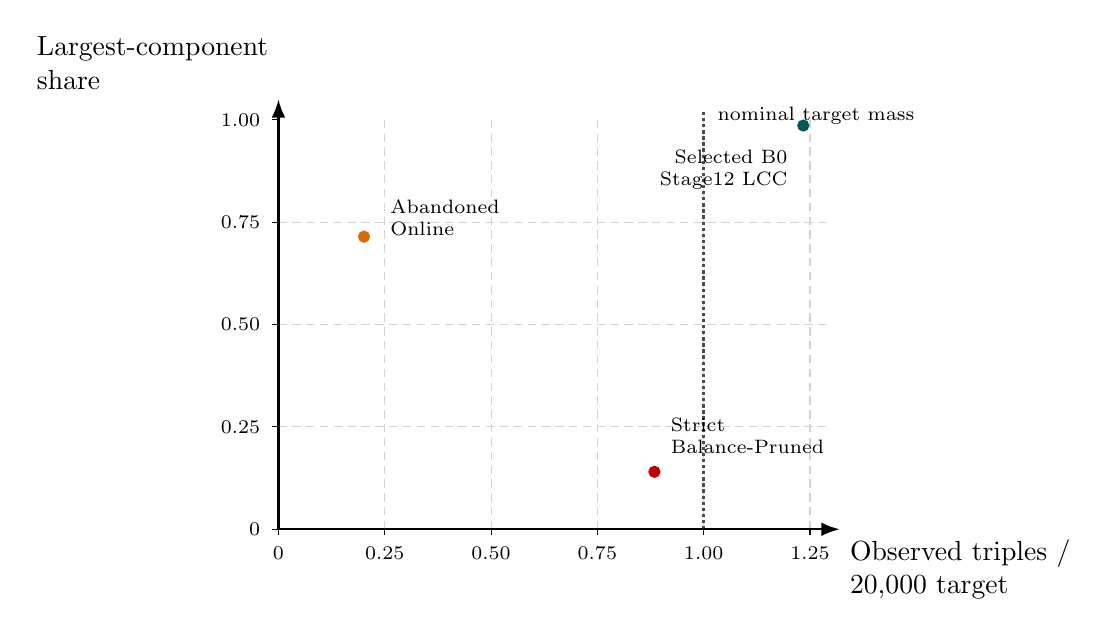
\begin{tikzpicture}[x=5.4cm,y=5.2cm,>=Latex]
    % Grid
    \draw[densely dashed, gray!35] (0,0.25) -- (1.3,0.25);
    \draw[densely dashed, gray!35] (0,0.50) -- (1.3,0.50);
    \draw[densely dashed, gray!35] (0,0.75) -- (1.3,0.75);
    \draw[densely dashed, gray!35] (0.25,0) -- (0.25,1.0);
    \draw[densely dashed, gray!35] (0.50,0) -- (0.50,1.0);
    \draw[densely dashed, gray!35] (0.75,0) -- (0.75,1.0);
    \draw[densely dashed, gray!35] (1.00,0) -- (1.00,1.0);
    \draw[densely dashed, gray!35] (1.25,0) -- (1.25,1.0);

    % Target line
    \draw[densely dotted, very thick, black!70] (1.0,0) -- (1.0,1.02);
    \node[font=\scriptsize, anchor=west] at (1.01,1.01) {nominal target mass};

    % Axes
    \draw[->, thick] (0,0) -- (1.32,0) node[below right, align=left] {Observed triples /\\20,000 target};
    \draw[->, thick] (0,0) -- (0,1.05) node[above left, align=left] {Largest-component\\share};

    % Ticks and labels
    \foreach \x/\lbl in {0/0,0.25/0.25,0.50/0.50,0.75/0.75,1.00/1.00,1.25/1.25} {
        \draw (\x,0) -- (\x,-0.015);
        \node[font=\scriptsize, anchor=north] at (\x,-0.02) {\lbl};
    }
    \foreach \y/\lbl in {0/0,0.25/0.25,0.50/0.50,0.75/0.75,1.00/1.00} {
        \draw (0,\y) -- (-0.015,\y);
        \node[font=\scriptsize, anchor=east] at (-0.02,\y) {\lbl};
    }

    % Points
    \filldraw[orange!85!black] (0.2013,0.7146) circle (2pt);
    \node[font=\scriptsize, align=left, anchor=west] at (0.24,0.76) {Abandoned\\Online};

    \filldraw[teal!70!black] (1.2342,0.9860) circle (2pt);
    \node[font=\scriptsize, align=right, anchor=north east] at (1.22,0.95) {Selected B0\\Stage12 LCC};

    \filldraw[red!75!black] (0.8842,0.1403) circle (2pt);
    \node[font=\scriptsize, align=left, anchor=south west] at (0.90,0.16) {Strict\\Balance-Pruned};
\end{tikzpicture}
\caption[Trade-off between fulfillment and structural coherence]{Trade-off between total realized mass and structural coherence across Abandoned Online, the selected B0 Stage12 largest component, and the strict balance-pruned ablation. The horizontal axis reports observed triples as a fraction of the nominal 20,000-triple target, while the vertical axis reports the share of entities contained in the largest connected component. The Abandoned Online point remains under-fulfilled but structurally more concentrated than the strict balance-pruned ablation, whereas B0 is structurally strongest but overfull. Because Abandoned Online was audited against an earlier allocation manifest, its horizontal position should be read as a broad fulfillment indicator rather than as a strict like-for-like benchmark against the later artifacts.}
\label{fig:tradeoff_fulfillment_connectivity}
\end{figure}





\subsection{Scope and Limitations}

% TODO before final submission if KGE results arrive:
% revise the fourth limit below so it distinguishes completed structural audit from newly added downstream evaluation.
The reported results should be interpreted within five limits. First, all pattern scores are empirical estimates over retrieved evidence under WDQS and cached intermediate artifacts; they are not logical guarantees over the full Wikidata graph. Second, composition discovery depends on weak semantic pruning signals, including incomplete Wikidata constraints and a conservative LLM-based target filter, so false negatives remain possible even though over-pruning was intentionally discouraged. Third, the selected B0 graph improves relation coverage more than perfect pattern-level balance: high-support taxonomic relations still exert strong pressure on connectivity and quota realization. B0 has higher surplus than later pruning candidates, and generic-relation dominance remains a limitation. Fourth, Abandoned Online was audited against an earlier allocation manifest than the later graph artifacts, so its exact fulfillment metrics are comparable only in broad terms rather than as a strict like-for-like target match. Fifth, in the present version, this work evaluates the benchmark-construction pipeline itself and emphasizes construction methodology and structural audit outcomes; downstream KGE experiments on the constructed benchmark are still ongoing. The final artifact package records hashes, metrics, and decision evidence, but full end-to-end reproducibility still depends on resolving environment details and upstream frozen-input provenance.

\section{Conclusion}
\label{sec:conclusion}

This work presented a two-phase methodology for structurally controlled benchmark construction from Wikidata under realistic query-budget and graph-construction constraints. Phase I identifies empirically supported relation patterns and converts them into relation-level quotas. Phase II uses those quotas as the reference for graph construction, repair, candidate comparison, and final artifact selection.

The evaluation shows why the online frontier-based strategy was not adopted as the final construction approach. It remained a shallow partial realization, whereas the selected B0 graph realizes all 139 allocated relations in a single weakly connected Stage12 repaired largest component containing 24,683 unique triples. At the same time, the final graph does not fully eliminate pattern imbalance: composition-heavy backbone relations remain overrepresented, showing that balance and connectivity remain competing objectives. Later Stage13/C1, C2, and \texttt{C3\_probe\_v1} analyses were treated as post hoc candidate analyses and did not supersede B0.

Future work should therefore focus on three directions:

\begin{itemize}
    % TODO before final submission if KGE results arrive:
    % replace the first item below with a short summary of the completed downstream evaluation.
    \item completing and integrating the ongoing downstream KGE evaluation on the constructed benchmark,
    \item reducing false negatives in composition-target pruning and verification, and
    \item strengthening controls for generic high-support relations without fracturing the graph.
\end{itemize}

\clearpage
\printbibliography

\end{document}
